% !TeX root = ../../thesis.tex
\chapter{Introduction}\label{ch:introduction}
This chapter presents an overview of non-valence anions, focusing on dipole-bound anions (DBAs). The significance of these anions in biological systems is explored, followed by an introduction to biological quinones and their crucial role in biological processes. Finally, the research objectives are outlined.

\section{Non-Valence Anions}
An anion is an atom or molecule possessing a negative charge. The binding of an additional electron to a neutral molecule is a balance between the attractive potential between the excess electron and the nuclei, and the repulsive forces from the electrons in the neutral molecule.  \cite{simons2008molecular,simons2023molecular,simons2011theoretical,herbert2015quantum}.

The binding energy of the excess electron is typically significantly lower than the ionisation energy of the neutral molecule. Morover, the propierties of the anion can be very diferent than of of the neutral secies, with differneces ranging from equilibrium structure to chemical reactivity. In discussions of molecular anions, the concept of electron affinity (EA) is key. The adiabatic electron affinity (AEA) quantifies the energy difference between a molecule and its corresponding anion, both in their structural ground state and lowest rovibrational levels. The vertical electron affinity (VEA), defined at the neutral equilibrium geometry, is particularly relevant for electron capture dynamics. A molecule with a positive EA is considered electronically stable, requiring energy input to remove an electron from the anionic state \cite{simons2008molecular}.

Molecular anions are classified into valence bound anions (VBA), where the excess electron occupies a compact orbital similar to valence molecular orbitals, and non-valence anions (NVA) \newglossaryentry{nva}{name={NVA},description={Non Valence Anion}}, where the excess electron occupies a diffuse orbital spatially separated from the molecule. Unlike valence electrons, these ``extra'' electrons do not experience a -1/r Coulombic attraction at long distances. Instead, they interact through weaker charge-multipole potentials, which are less robust than the covalent bonds holding the molecule together\cite{simons2008molecular,herbert2015quantum}.

Non-valence anions can be categorised into dipole-bound states (DBSs)\cite{fermi1947capture,wallis1960energy,desfranccois1996abdoul,gutowski1996contribution,jordan2003theory,qian2019probing,gulania2020quest,yuan2020observation,slimak2022binding,yuan2023observation}, quadrupole-bound states (QBSs)\cite{jordan1979binding,desfranccois2004long,sommerfeld2014excess,zhu2017observation,liu2019ground,liu2020observation}, and correlation-bound states (CBSs)\cite{sommerfeld2010correlation,bezchastnov2011anions,voora2013existence,voora2014nonvalence,voora2015nonvalence,voora2017theoretical,ciborowski2019correlation,krafft2022perfluorocubane}.
In DBSs, the excess electron is stabilised by the interaction with the molecule's significant dipole moment. It is generally accepted that a dipole moment of approximately 2.5 D is required to bind an extra electron\cite{jordan2003theory}, although having a dipole moment above this threshold does not guarantee the formation of a dipole-bound anion. QBSs, on the other hand, arise from electrostatic interactions involving a large quadrupole moment in molecules with no dipole moment. Unlike DBSs, no definitive critical quadrupole moment has been established for the formation of quadrupole-bound states\cite{sommerfeld2014excess}. Lastly, CBSs are stabilised not by electrostatic forces but by dispersion interactions. It is worth noting that many DBSs and QBSs remain unbound if electron correlation effects are ignored, which blurres the distinction between these types of non-valence anions\cite{voora2017theoretical}. Examples of different anion types are shown in Figure \ref{fig:AnionTypes}.

\begin{figure}[h]
  \centering
  \begin{minipage}[b]{0.27\textwidth}
    \centering
    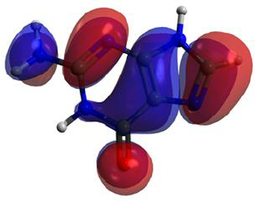
\includegraphics[width=\textwidth]{chapters/introduction/image/vbaDNA.png}
    \small\emph{Valence anion}
  \end{minipage}
  \hfill
  \begin{minipage}[b]{0.30\textwidth}
    \centering
    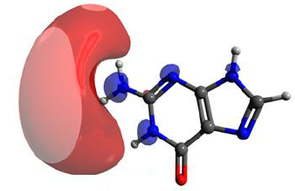
\includegraphics[width=\textwidth]{chapters/introduction/image/dbaDNA.png}
    \small\emph{Dipole-bound anion}
  \end{minipage}
  \hfill
  \begin{minipage}[b]{0.27\textwidth}
    \centering
    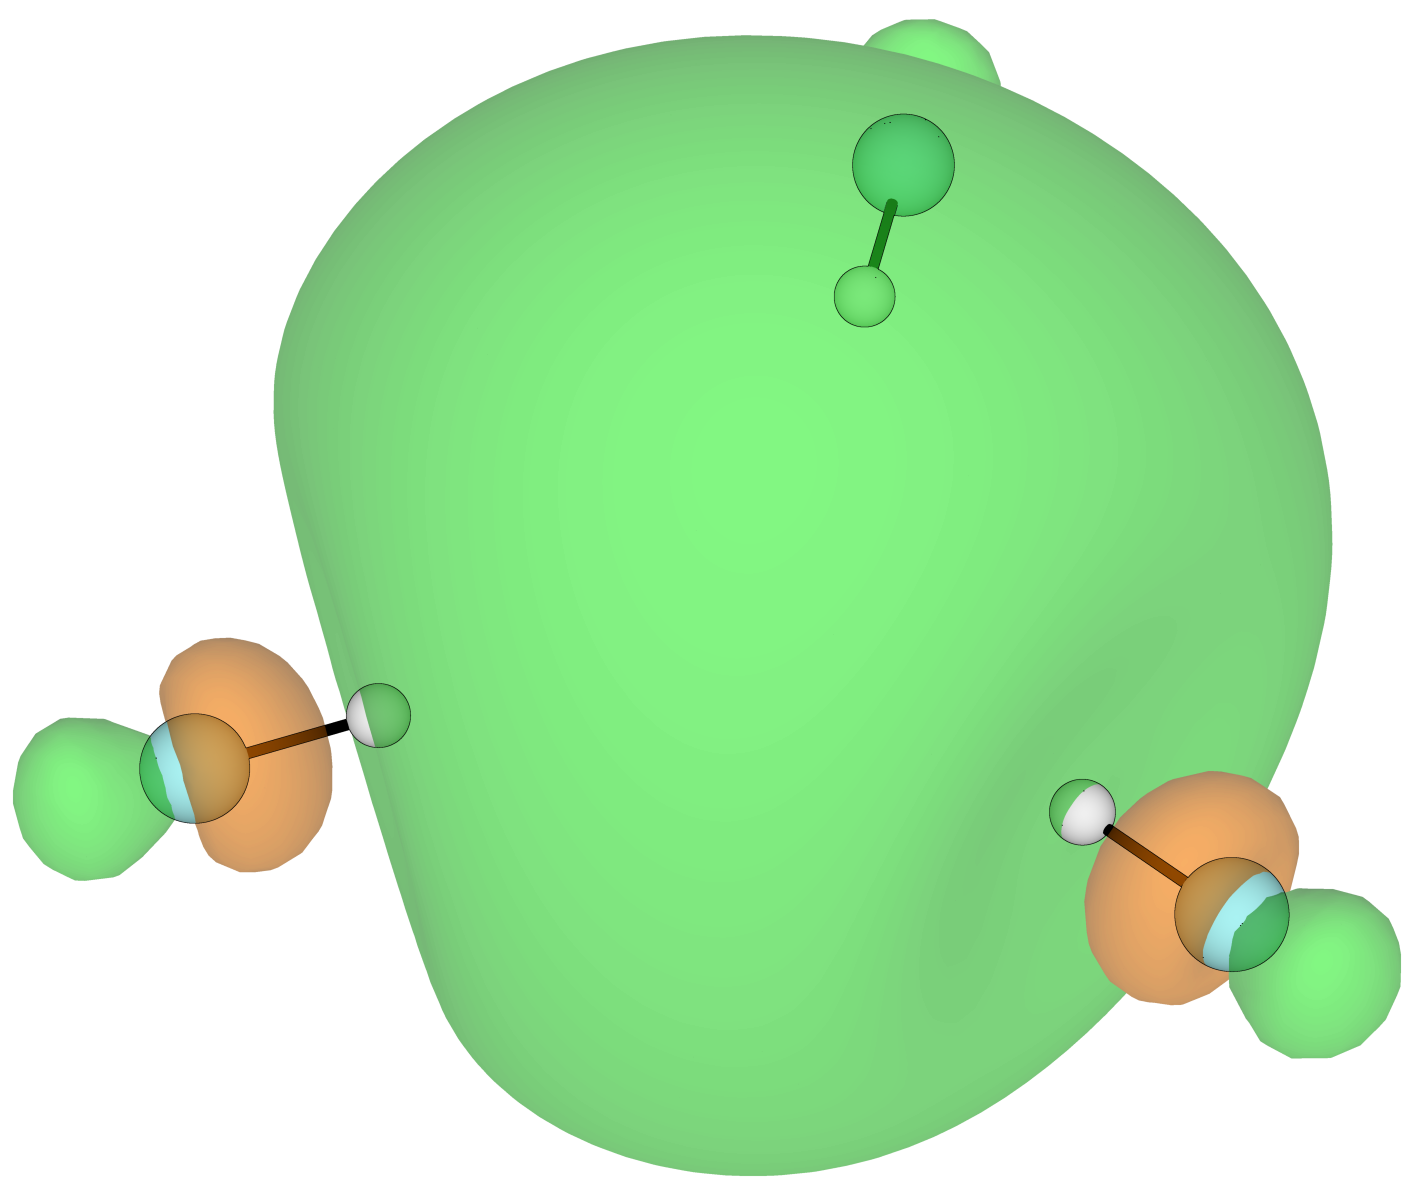
\includegraphics[width=\textwidth]{chapters/introduction/image/hf3.png}
    \small\emph{(HF)\textsubscript{3} solvated electron}
  \end{minipage}
  \caption[Valence and Non-Valence Anions]{Valence and Non-Valence Anions, a) and b) are reproduced from \cite{dutta2015electron}, c) from \cite{jordan2003theory}. \textbf{I will substitute by my own figs}}
  \label{fig:AnionTypes}
\end{figure}

\subsection{Dipole-Bound Anions}
Of the different non-valence anions, DBSs are the most common and well-studied. They were first proposed in 1947, where it was demostrated that a dipole could bind an excess electron if the dipole moment exceeds 1.6 D \cite{fermi1947capture}. Further investigations refined this concept for "real" molecules, leading to a critical dipole moment of approximately 2.5 D \cite{jordan2003theory}.

The weak forces that bind the excess electron are responsible for the diffuse nature of the state, with the electronic density often extending several Å away from the nuclei, and their relatively low binding energy, usually below 0.1 eV. This makes them susceptible to external perturbations, such as solvent interactions or external electric fields, which can significantly influence their stability and reactivity \cite{schiedt1998anion,hall2002two,jalbout2001dipole,gutowski2002solvated,skurski2002excess,jordan2003theory,eustis2007photoelectron,simons2008molecular,herbert2015quantum,clarke2025role}

Despite their binding energy being comparable to thermal energy ($k_bT\,\sim\,23$ meV), which might suggest limited practical relevance due to potential detachment, DBAs can play a significant role in systems that support both VBAs and NVAs. These systems can undergo a transition from a non-valence anion state to a stable valence state \cite{herbert2015quantum,jordan2003theory}. Moreover, since the electron density of an NVA is spatially extended and resides far from the nuclei, the relaxed structure of an NVA is much closer to that of the neutral molecule compared to a VBA. This large spatial extent also results in a higher cross-section for electron capture and transfer. Consequently, DBSs can act as "doorway" states, facilitating electron capture and transfer processes \cite{hendricks1998dipole,desfrancois1999electron,sommerfeld2002coupling,jordan2003theory,sommerfeld2004intramolecular,sommerfeld2005dipole,sommerfeld2007doorway,simons2008molecular,verlet2020role,kang2022state,hassan2022associative,simons2023molecular,kang2024reaction}. This unique behavior has sparked interest in the role of NVAs across various fields, including astrochemistry \cite{fortenberry2015interstellar,millar2017negative} and radiobiology \cite{gu2012interactions,narayanan2023secondary,sedmidubska2024interaction}.

\subsection{Approaches to Study Non-Valence Anions}
Significant progress has been made in experimental and theoretical methods for elucidating the structure and dynamics of NVAs. \cite{desfranccois1995determination,simons2008molecular,simons2023molecular,clarke2024dynamics} Experimentally, dipole-bound anions are characterised using spectroscopic techniques designed to probe their weakly bound electronic states \cite{rienstra2002atomic,liu2020photoelectron,simons2008molecular,rogers2019photoelectron,clarke2024dynamics}. In photodetachment and photoelectron spectroscopies, a beam of the target species is generated—often using a laser vaporisation or electrospray source—and probed with light. The energy of the ejected electrons reveals information about the electron binding energy and electronic structure. Time-resolved photoelectron spectroscopy (TRPES)\cite{cyr1996femtosecond,neumark2001time,stolow2004femtosecond,wu2011time,schuurman2022time} extends this approach, using ultrafast laser pulses to investigate the dynamics of electron attachment and detachment on femtosecond timescales, revealing transient states and relaxation pathways. DBSs can also be accessed by Rydberg electron transfer spectroscopy (RET)\cite{carles2001rydberg,eustis2007photoelectron,bradforth2002excited}, which has been used to probe their role in electron transfer dynamics. Time-of-flight mass spectrometry is often coupled with these techniques to identify and isolate the correct anionic species \cite{desfranccois1996abdoul,liu2019ground,ameixa2023parent,pshenichnyuk2020ionizing}.

The theoretical investigation of DBAs presents two main challenges. Firstly, the large spatial extent of the DB orbital requires atomic orbital basis sets that are sufficiently diffuse to accurately describe it, necessitating the use of large custom basis sets \cite{skurski2000choose}. Secondly, electron correlation is important; although the electron density at the valence level remains largely unchanged from the parent molecule, the diffuse part of the density, corresponding to the DB state, is considerably polarisable due to its diffuse nature and exhibits significant dispersion-like interactions with the valence region, contributing substantially to the binding energy of the extra electron \cite{simons2008molecular,simons2011theoretical,simons2023molecular,gutowski1996contribution,voora2017theoretical}.

Regarding computational methods, standard density functional theory (DFT) approaches can fail because most exchange-correlation functionals cannot properly describe dispersion interactions and can suffer from spin contamination in open-shell molecules \cite{thiam2023accurately}. Multiconfigurational methods like complete active space self-consistent field (CASSCF)\cite{vila2002theoretical,ivanov2015anion} can capture the static correlation nature of the open shell systems, but require considerable effort in selecting an appropriate active space that balances accuracy and computational feasibility. Morover, they lack dynamic correlation inherent in the dispersion. Currently, equation-of-motion coupled-cluster (EOM-CC)\cite{herbert2015quantum,jordan2003theory,moorby2024signatures} methods are often used for DBA modelling as they adequately treat both the electron correlation and open-shell character. However, the high computational cost of EOM-CC approaches significantly limits their applicability to larger molecular systems. To address this, some approximate methods have been developed, such as the second order approximate CC \cite{christiansen1995second,paran2024performance}- which is used in this work, or the domain-based local pair natural orbital coupled-cluster theory (DLPNO) method\cite{haldar2020multilayer,schulz2018systematic}.

\subsection{Non-Valence Anions in Condensed Matter}

Several studies have indicated that the presence of individual molecules interacting with a molecule supporting an NVA can further stabilise the state by increasing the total dipole moment, or by combining individual dipoles to collectively bind the electron in a intermolecular cabity. The excess electron is stabilised by the interaction with multiple solvent molecules, rather than binding to any individual molecule, and is known as a solvated electron \cite{schiedt1998anion,hall2002two,jalbout2001dipole,gutowski2002solvated,skurski2002excess,jordan2003theory,eustis2007photoelectron,simons2008molecular,herbert2015quantum,clarke2025role}

The binding energy of such solvated electrons can increase dramatically with cluster size. A water molecule does not support any bound anionic state\cite{herbert2015quantum}, however a water dimer anion (H\textsubscript{2}O)\textsubscript{2}\textsuperscript{-} exhibits a very low vertical detachment energy (VDE) of only 0.045 eV\cite{coe1990photoelectron,lee1991negative}. Water cluster anions (H\textsubscript{2}O)\textsubscript{n}\textsuperscript{-} made of \emph{ca.} 100 molecules can achieve VDEs exceeding 2.0 eV\cite{verlet2005observation,ma2009low}, and in bulk this values is measured to be higher than between 3.4 and 4 eV\cite{ma2009low,coe2008photoelectron,siefermann2010binding}. The structure of the state was subject of much debate in the literature \cite{herbert2017hydrated,kumar2015simple,herbert2019structure,herbert2017hydrated,kevan1981solvated}, but it is now generally accepted that the excess electron resides in a cavity of approximately 2.5 \r{A} in size \cite{herbert2017hydrated,herbert2019structure}. This example shows how weakly bound non-valence state can transform into a strongly bound electronic species, though with significantly altered properties. 

For solutes, the existence of a hydrated NVAs is still remains a subject of discussion \cite{anusiewicz2020fate,castellani2019stability,larsen2010does}. Computational studies suggest that hydration influences the localisation of the excess electron, often displacing it onto the solvent cage's surface \cite{anusiewicz2020fate}. Conversely, experimental evidence indicates that alkyl chains do not disrupt DBS stability \cite{castellani2019stability}, and DBS-mediated mechanisms have been observed in solvated uracil systems \cite{narayanan2024electron}. The viability of NBS in bulk systems depends on the molecular density and polarity of the medium. While solvents may hinder DBS existence due to excluded volume effects, they can also stabilise DBS through Van der Waals interactions \cite{bradforth2002excited,chen2000precursors}. Distinct scenarios can be considered in the interaction between a DBA supporting molecule and solvent: the electron may be localised in the NVA orbital, captured by the solvent to form a cage, or interact with solvent molecules whose dipole can orient to stabilise the DB state. The latter two phenomena are linked to charge-transfer-to-solvent (CTTS) electronic transitions and are observed experimentally \cite{staib1996reaction,chen2000precursors,bradforth2002excited,chen2008ultrafast,messina2013real,carter2023birth,lan2024dynamics}.

\subsection{Non-Valence Anions in Biological Systems}

Research on dipole-bound anions (DBAs) has predominantly focused on gas-phase systems. However, in biological contexts, DBAs have garnered attention for their interactions with DNA, particularly in the context of radiation-induced damage and radiosensitizers \cite{gu2012interactions,narayanan2023secondary,sedmidubska2024interaction}.
When high-energy radiation interacts with biological samples, it generates a cascade of secondary electrons which can be captured by cellular constituents, potentially through non-valence states. It has been hypothesized that NVAs supported by DNA act as electron scavengers, leading to strand breaks and other forms of damage \cite{gu2012interactions,narayanan2023secondary,dutta2015electron,narayanan2024electron,sommerfeld2005dipole}.
Radiosensitizers are drugs designed to enhance the efficacy of radiation therapy in cancer treatment. These compounds become cytotoxic upon capturing secondary electrons generated during radiation exposure, potentially through the formation of NVAs \cite{sedmidubska2024interaction}.

The role of NVAs in natural biological pathways beyond genetic damage remains largely unexplored. It has been proposed that vacant pockets in proteins could accommodate non-valence states \cite{castellani2019stability}. Enzymes play a crucial role in almost all biological reactions, particularly in the transfer and transport of electrons through biological matter. These processes are central to vital phenomena such as photosynthesis \cite{mitchell1961coupling}, aerobic respiration \cite{wikstrom1977proton}, and biological nitrogen fixation \cite{rutledge2020electron}. The range of these electron transfers is remarkable, spanning timescales from picoseconds to milliseconds and distances between donor and acceptor molecules from a few to over hundreds of angstroms \cite{gray1996electron,blumberger2015recent}. Long-range electron transport is typically achieved through a chain of cofactors, often metal clusters, which facilitate a stepwise transfer of the electron. The inter-cluster distances range from a few angstroms to over 20 \r{A}. To model these transfer reactions, it is commonly assumed that the electron tunnels between the donor and acceptor. Specifically, in the Superexchange model, the tunnelling process is mediated by unoccupied orbitals in the intervening space, effectively lowering the tunnelling barrier \cite{blumberger2015recent}. The sensitivity of non-valence anion states to environmental factors suggests a potential and elegant mechanism that natural systems could exploit to regulate long-range electron transfer processes.

In this study, we aim to focus on other biological targets, which could use an interplay between NVAs and VBAs. A compound that is ubiquitous in nature and relevant to electron transfer in proteins is ubiquinone.

\iffalse DBAs have been used as the explanaiton for the presence of methil functional groups electron of flavins \cite{matthews2018observation}; they would disrupt that state, making the \fi

\section{Ubiquinone}
Quinones, named for the bark of the cinchona tree from which it was isolated in the 18th century \cite{rusell1873quinone}, are a class of organic compounds with a fully conjugated cyclic dione structure derived from aromatic compounds by conversion of an even number of C-H to ketone groups \cite{IUPACQ050152025}. Quinones are known for their redox properties and play crucial roles in various biological processes, including electron transport in cellular respiration and photosynthesis \cite{ernster1995biochemical,chen2024low}.

\begin{figure}[ht!]
  \centering
  \begin{tikzpicture}[x=1pt,y=1pt]
    \node at (130,0) {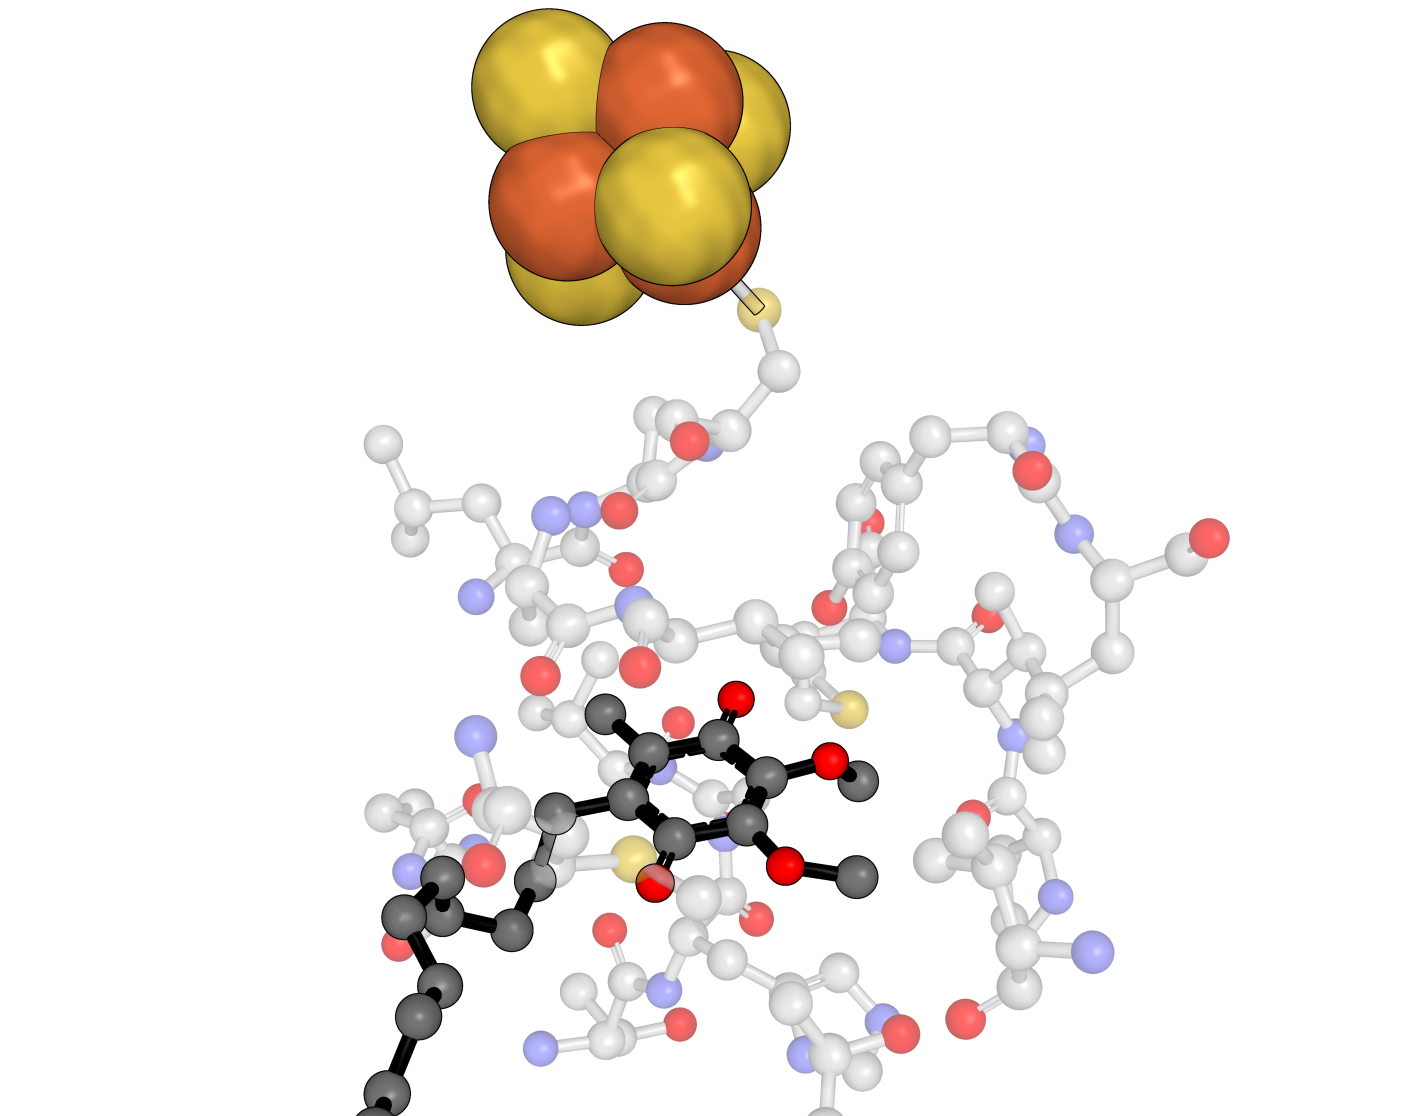
\includegraphics[width=0.45\textwidth]{chapters/introduction/image/uQ_6i0d.png}};
    \node at (215,35) {\includegraphics[width=0.25\textwidth]{chapters/introduction/image/Ubiquinone–ubiquinol_conversion.svg.png}};
    \node at (0,0) {\includegraphics[width=0.47\textwidth]{chapters/introduction/image/Mitochondrial_electron_transport_chain—Etc4.svg.png}};
  \end{tikzpicture}
  \caption[Role of ubiquinone]{Roles of Ubiquinone. Left; electron transport chain in the mitocondria, ubiquinones get reduced at complexes I and II and reduced at complex III. Center: Q\textsubscript{10} at the active site of the bacterial complex I (PDB: 6i0d) \cite{gutierrez2020key}. Right: Ubiquinone to ubiquinol interconversion.}
  \label{fig:ETC}
\end{figure}

This work focuses on ubiquinone -\textit{ubi} from being ubiquitous in nature-, also known as coenzyme Q (CoQ), a lipid-soluble molecule that exists as a quinone or quinol, then named ubiquinol. It plays a role in aerobic respiration in the electron transport chain (ETC) as an electron carrier, accepting 2 electrons at complexes I or II and donating them in complex III\cite{ernster1995biochemical}. In Figure \ref{fig:ETC}, a schematic of the ETC is presented.

Ubiquinone is composed of a benzoquinone ring, 2,3-dimethoxy-6-methyl-p-benzoquinone, and a long side chain, composed of a variable number of isoprenoid units depending on the organism, 10 in humans. This number, \textit{n}, is used for the naming of the specific ubiquinone (Q\textsubscript{n}). In Figure \ref{fig:QuinoneTypes} different Q\textsubscript{n} are presented. The benzoquinone moiety is responsible for its redox properties, while the isoprenoid tail enhances its lipid solubility, allowing it to integrate into biological membranes. \cite{ernster1995biochemical}.

\begin{figure}[ht!]
  \centering
  \begin{tikzpicture}[anchor=south west, x=1cm, y=1cm]
    \node (img1) at (0,20pt) {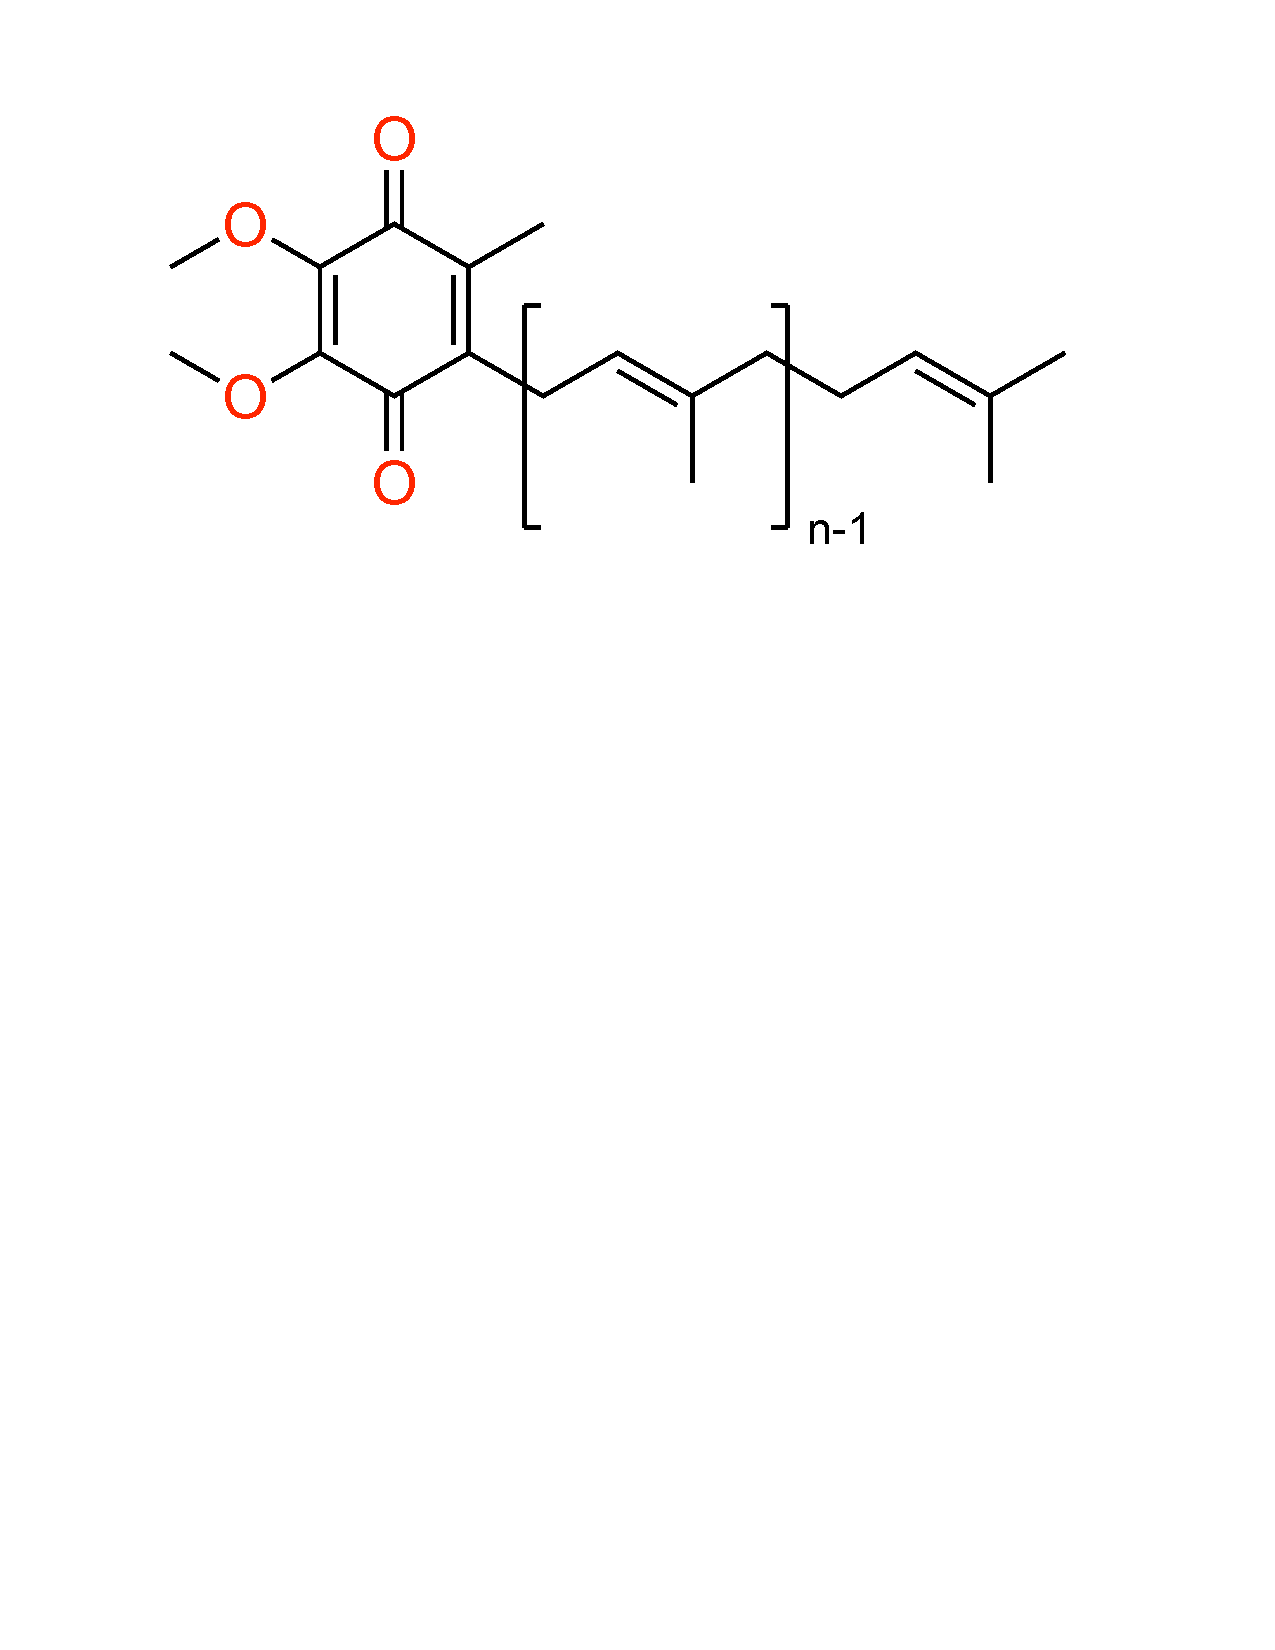
\includegraphics[width=0.45\textwidth]{chapters/introduction/image/UQ_Struct.pdf}};
    \node (img2) at (0.39\textwidth,0) {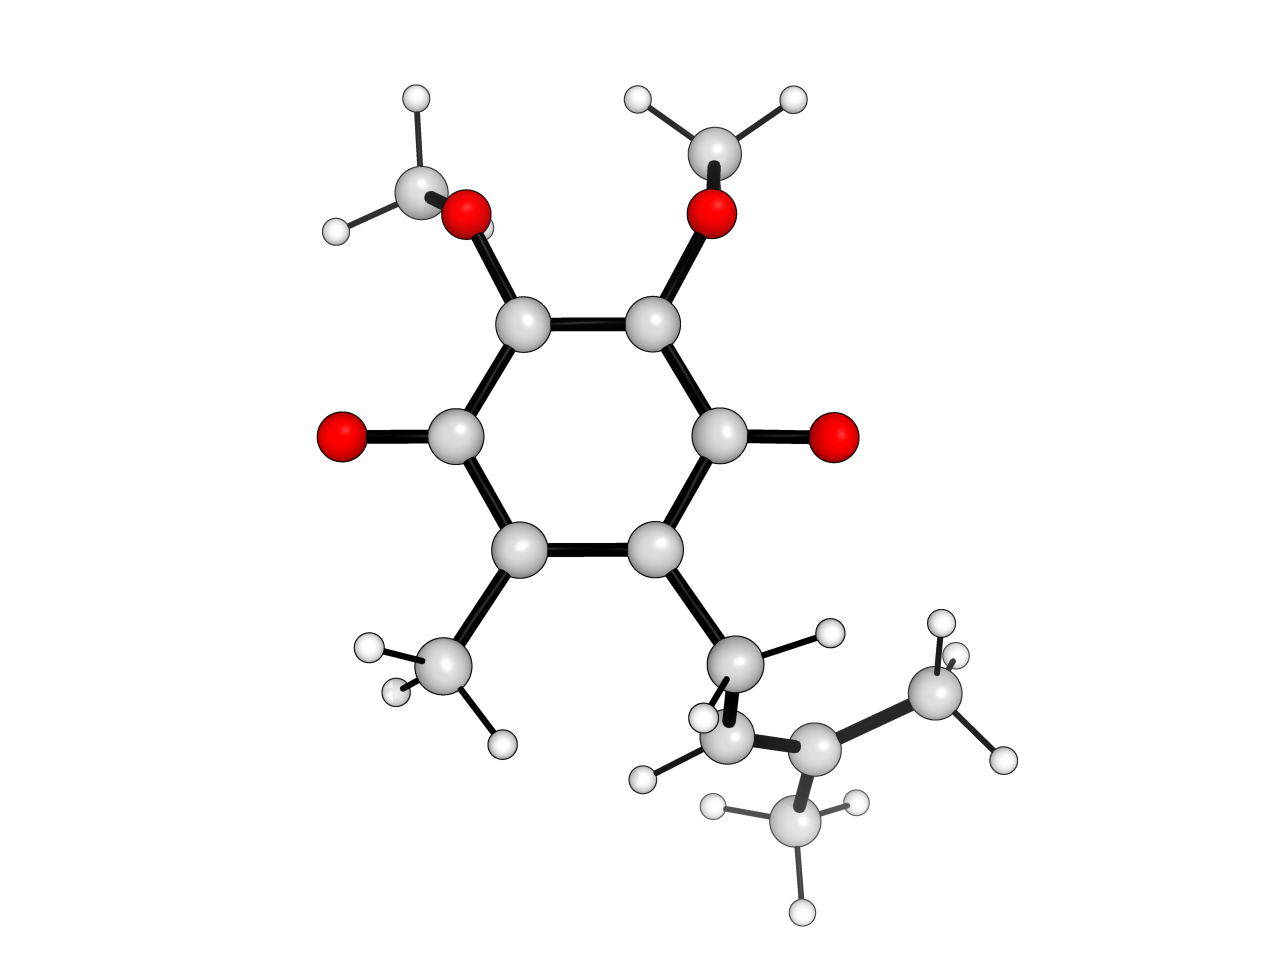
\includegraphics[width=0.4\textwidth]{chapters/introduction/image/Q1.png}};
    \node (img3) at (0.66\textwidth,0) {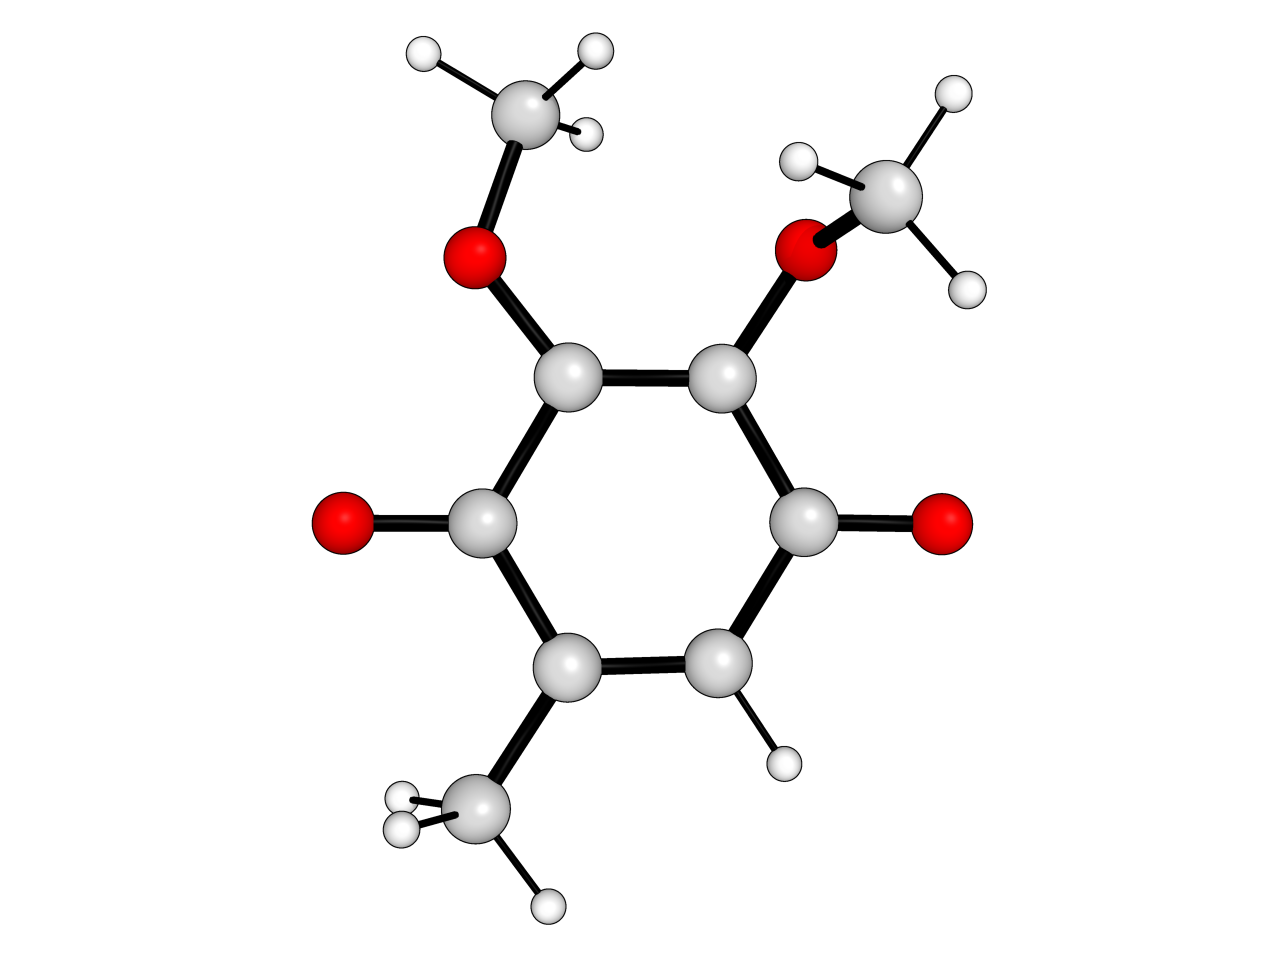
\includegraphics[width=0.4\textwidth]{chapters/introduction/image/Q0189.png}};
    \node[align=center, text=darkgray] at ([yshift=-28pt, xshift=-1.2cm]img1.south) {\footnotesize General structure of CoQ};
    \node[align=center, text=darkgray] at ([yshift=-8pt]img2.south) {\footnotesize Q1};
    \node[align=center, text=darkgray] at ([yshift=-8pt]img3.south) {\footnotesize Q0};
  \end{tikzpicture}
  \caption[Quinone structures]{Quinones used in this work. From left to right: Q\textsubscript{0}, Q\textsubscript{1}, Q\textsubscript{10} in the enzyme PDB bla bla.}
  \label{fig:QuinoneTypes}
\end{figure}

The ubiquinone moiety can support two types of anion states, a VBA and a DBA. In p-benzoquinone, the valence anion can be understood from the H{\"u}ckel picture with the excess electron with the excess electron occupying a vacant \textpi \textsuperscript{*} orbital. This state is stabilised relative to benzene thanks to the electron withdrawing ketone groups. In ubiquinone, the VBA is bound with an energy of around of 1.7 eV \cite{chen2024low}. The dipole-bound anion, on the other hand, results from the two methoxy chains, whose configuration mainly controls the dipole of the molecule \cite{ameixa2023parent}. The interplay between these functional groups, especially in the case of Q\textsubscript{0}, without the flexible isoprenoid tail, makes it a very interesting system to study. It is a fairly rigid molecule, except for the dihedral angles between the methoxy groups and the benzoquinone ring. Their configuration will affect the dipole moment and could therefore determine the existance and energetics of the DBA \cite{ameixa2023parent,bull2015anion}. This allows the study of a fairly complicated electronic structure in terms of two coordinates.

When the isoprenoid tail is considered, it has been shown that it further stabilises the valence anion \cite{pshenichnyuk2020ionizing}. Its effects on the dipole state have not been studied. One can imagine the effect for to be moderate for shorter tails; it will slightly modify the dipole moment of the system, but structurally it will be quite far from the orbital occupied by the excess electron. For longer tails, the isoprenoid chain could sterically hinder the dipole-bound state.

There have been extensive studies on the electron binding properties of the ubiquinone family, both experimentally \cite{ameixa2023parent,west2014anion,pshenichnyuk2020ionizing,bull2015anion} and theoretically \cite{ameixa2023parent,pshenichnyuk2020ionizing,haldar2020multilayer, nonella1998quantum, gamiz2017terminal}. However, these studies have been centred on understanding the valence anion of the quinone, and no comprehensive study of its dipole bound state has been performed; the VBA is the final acceptor of the electron and the existence of the DBA in condensed phase is dubious.
However, experimental studies have observed dipole-bound anions in the gas phase in ubiquinones Q\textsubscript{0} and Q\textsubscript{1} \cite{ameixa2023parent} with an EA of $\mathrm{\sim}$60 meV. Although its signal is reduced as more isoprenoid units are added, interpreted as an effect of the isprenoid tail being flexible and resulting in a steric hindrance of the state \cite{ameixa2023parent,pshenichnyuk2020ionizing}, one could imagine that in a protein moiety, the geometry of the tail would be fixed far from a potential DB orbital, which could even be further stabilised by residues pointing in the cavity. This motivates the current study.

The main objective of this work is to study the dipole-bound anion of ubiquinone. We use the electron attachemnt variant of equation-of-motion CC2 (EA-EOM-CC2), which has recently shown to be effective in dipole bound states of organic molecules \cite{paran2024performance}. The specific objectives are:
\begin{itemize}
  \item Benchmark the effectiveness of the EA-EOM-CC2 method to compute the electron affinity of quinones.
  \item Implement the Dyson orbital approach for EOM-CC2, for better characterisation.
  \item To investigate the dipole-bound anion of ubiquinone in terms of its functional group configurations.
  \item To study the effect of the protein environment on the dipole-bound anion of ubiquinone, treated as a cluster model using small molecules.
\end{itemize}

\iffalse \begin{figure}[th!]
  \centering
  % GNUPLOT: LaTeX picture with Postscript
\begingroup
  \makeatletter
  \providecommand\color[2][]{%
    \GenericError{(gnuplot) \space\space\space\@spaces}{%
      Package color not loaded in conjunction with
      terminal option `colourtext'%
    }{See the gnuplot documentation for explanation.%
    }{Either use 'blacktext' in gnuplot or load the package
      color.sty in LaTeX.}%
    \renewcommand\color[2][]{}%
  }%
  \providecommand\includegraphics[2][]{%
    \GenericError{(gnuplot) \space\space\space\@spaces}{%
      Package graphicx or graphics not loaded%
    }{See the gnuplot documentation for explanation.%
    }{The gnuplot epslatex terminal needs graphicx.sty or graphics.sty.}%
    \renewcommand\includegraphics[2][]{}%
  }%
  \providecommand\rotatebox[2]{#2}%
  \@ifundefined{ifGPcolor}{%
    \newif\ifGPcolor
    \GPcolortrue
  }{}%
  \@ifundefined{ifGPblacktext}{%
    \newif\ifGPblacktext
    \GPblacktexttrue
  }{}%
  % define a \g@addto@macro without @ in the name:
  \let\gplgaddtomacro\g@addto@macro
  % define empty templates for all commands taking text:
  \gdef\gplbacktext{}%
  \gdef\gplfronttext{}%
  \makeatother
  \ifGPblacktext
    % no textcolor at all
    \def\colorrgb#1{}%
    \def\colorgray#1{}%
  \else
    % gray or color?
    \ifGPcolor
      \def\colorrgb#1{\color[rgb]{#1}}%
      \def\colorgray#1{\color[gray]{#1}}%
      \expandafter\def\csname LTw\endcsname{\color{white}}%
      \expandafter\def\csname LTb\endcsname{\color{black}}%
      \expandafter\def\csname LTa\endcsname{\color{black}}%
      \expandafter\def\csname LT0\endcsname{\color[rgb]{1,0,0}}%
      \expandafter\def\csname LT1\endcsname{\color[rgb]{0,1,0}}%
      \expandafter\def\csname LT2\endcsname{\color[rgb]{0,0,1}}%
      \expandafter\def\csname LT3\endcsname{\color[rgb]{1,0,1}}%
      \expandafter\def\csname LT4\endcsname{\color[rgb]{0,1,1}}%
      \expandafter\def\csname LT5\endcsname{\color[rgb]{1,1,0}}%
      \expandafter\def\csname LT6\endcsname{\color[rgb]{0,0,0}}%
      \expandafter\def\csname LT7\endcsname{\color[rgb]{1,0.3,0}}%
      \expandafter\def\csname LT8\endcsname{\color[rgb]{0.5,0.5,0.5}}%
    \else
      % gray
      \def\colorrgb#1{\color{black}}%
      \def\colorgray#1{\color[gray]{#1}}%
      \expandafter\def\csname LTw\endcsname{\color{white}}%
      \expandafter\def\csname LTb\endcsname{\color{black}}%
      \expandafter\def\csname LTa\endcsname{\color{black}}%
      \expandafter\def\csname LT0\endcsname{\color{black}}%
      \expandafter\def\csname LT1\endcsname{\color{black}}%
      \expandafter\def\csname LT2\endcsname{\color{black}}%
      \expandafter\def\csname LT3\endcsname{\color{black}}%
      \expandafter\def\csname LT4\endcsname{\color{black}}%
      \expandafter\def\csname LT5\endcsname{\color{black}}%
      \expandafter\def\csname LT6\endcsname{\color{black}}%
      \expandafter\def\csname LT7\endcsname{\color{black}}%
      \expandafter\def\csname LT8\endcsname{\color{black}}%
    \fi
  \fi
    \setlength{\unitlength}{0.0500bp}%
    \ifx\gptboxheight\undefined%
      \newlength{\gptboxheight}%
      \newlength{\gptboxwidth}%
      \newsavebox{\gptboxtext}%
    \fi%
    \setlength{\fboxrule}{0.5pt}%
    \setlength{\fboxsep}{1pt}%
    \definecolor{tbcol}{rgb}{1,1,1}%
\begin{picture}(4600.00,4320.00)%
    \gplgaddtomacro\gplbacktext{%
      \csname LTb\endcsname%%
      \put(714,562){\makebox(0,0)[r]{\strut{}$-1.5$}}%
      \csname LTb\endcsname%%
      \put(714,1156){\makebox(0,0)[r]{\strut{}$-1$}}%
      \csname LTb\endcsname%%
      \put(714,1749){\makebox(0,0)[r]{\strut{}$-0.5$}}%
      \csname LTb\endcsname%%
      \put(714,2343){\makebox(0,0)[r]{\strut{}$0$}}%
      \csname LTb\endcsname%%
      \put(714,2936){\makebox(0,0)[r]{\strut{}$0.5$}}%
      \csname LTb\endcsname%%
      \put(714,3530){\makebox(0,0)[r]{\strut{}$1$}}%
      \csname LTb\endcsname%%
      \put(714,4124){\makebox(0,0)[r]{\strut{}$1.5$}}%
      \csname LTb\endcsname%%
      \put(812,386){\makebox(0,0){\strut{}$-10$}}%
      \csname LTb\endcsname%%
      \put(1680,386){\makebox(0,0){\strut{}$-5$}}%
      \csname LTb\endcsname%%
      \put(2549,386){\makebox(0,0){\strut{}$0$}}%
      \csname LTb\endcsname%%
      \put(3417,386){\makebox(0,0){\strut{}$5$}}%
      \csname LTb\endcsname%%
      \put(4286,386){\makebox(0,0){\strut{}$10$}}%
    }%
    \gplgaddtomacro\gplfronttext{%
      \csname LTb\endcsname%%
      \put(3530,3965){\makebox(0,0)[r]{\strut{}$\sin(x)$}}%
      \csname LTb\endcsname%%
      \put(3530,3789){\makebox(0,0)[r]{\strut{}$\cos(x)$}}%
      \csname LTb\endcsname%%
      \put(3530,3613){\makebox(0,0)[r]{\strut{}$\tan(x)$}}%
      \csname LTb\endcsname%%
      \put(161,2343){\rotatebox{-270.00}{\makebox(0,0){\strut{}$y$}}}%
      \csname LTb\endcsname%%
      \put(2549,123){\makebox(0,0){\strut{}$x$}}%
    }%
    \gplbacktext
    \put(0,0){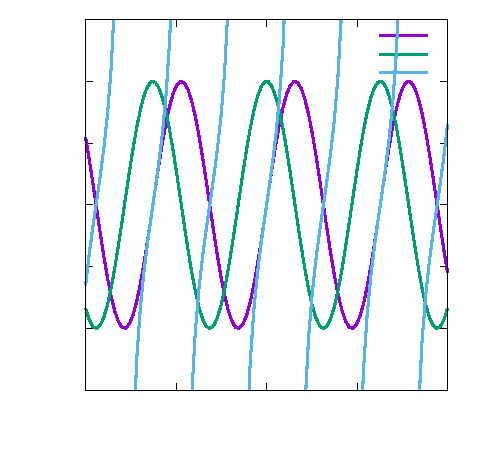
\includegraphics[width={230.00bp},height={216.00bp}]{test}}%
    \gplfronttext
  \end{picture}%
\endgroup

  %figsize is set in image/test.gp 
  \caption[Short caption for Table of Figures]{Illustration of how to
  include a figure (long text, should not go to Table of Figures).}
  \label{fig:test}
\end{figure} \fi

%%%%%%%%%%%%%%%%%%%%%%%%%%%%%%%%%%%%%%%%%%%%%%%%%%
% Keep the following \cleardoublepage at the end of this file, 
% otherwise \includeonly includes empty pages.
\cleardoublepage

% vim: tw=70 nocindent expandtab foldmethod=marker foldmarker={{{}{,}{}}}
